Some published numerical experiments have over time become benchmarks for other codes, while some 
others showcased comparisons between codes. Here is a short list of 'famous' benchmarks' in the 
computational geodynamics community.

\begin{itemize}
\item the plastic brick \cite{lemm08,kaus10,qurj09,mishin11,maie12,spmw16,gltf18,frbt19}
\item 2D Rayleigh-Benard convection (Blankenbach)  \cite{blbc89,trha98,chhl08,king09,lezh11,vyrc13,trab90,bepo10}
\item 2D Rayleigh-Taylor convection/instability \cite{pros81,trab90,wesc92,popo92,soga01,bast02,taki03,bomh06, basd08,qurj09,saev10,como97,lezh11,lomw12,vyrc13,vaks97,bomh06,chtl13,deka08,mishin11,maie12,fusc13,devv00a,dadh07,demh19}
\item 3D Rayleigh-Taylor instability \cite{fukk08,vosc15}
\item subduction problems \cite{scbe08,vack08,cehg14}
\item numerical sandbox \cite{bbeg06,maie12,busa16,gltf18}
\item the Stokes sphere \cite{galemanual}, in visco-plastic fluid \cite{bemj04}
\item the sinking block (sinker) \cite{thie11,cehg14,gery10,geyu03,mamo08,mishin11,fumt11,maie12} (see Section~\ref{sec:sinker})
\item multiple sinkers \cite{mabl14,mabl15}
\item 2D compressible Stokes flow problem \cite{itki94,tagu07,lezh08,kilv10,lizh13}
\item 3D convection at infinite Prandtl number (Busse) \cite{bucc93,trha98,omma06,krhb12}
\item Free surface evolution \cite{crsg12}
\item Love's problem \cite{bebe04}
\item Poiseuille flow \cite{fojg94,fuku11,tagm09}
\item Couette flow with temperature dependent viscosity \cite{egat10,demh19}
\item Couette flow with shear heating \cite{egat10}
\item Poiseuille-Couette flow \cite{fusc13}
\item Lid driven Cavity \cite{foth79,ghgs82,bope98,kawa61,brsa06}
\item Wannier flow \cite{wann50,yemu99,cehg14}
\item bending of elastic plate/beam \cite{cehg14,boht08a,vosc15,egat10,demh19}
\item flexure of finite length elastic plate \cite{chtl13}
\item thermal diffusion of half-cooling space \cite{chtl13}
\item stress build-up in Maxwell visco-elastic material \cite{geyu07,chtl13,egat10,demh19}
\item plastic oedometer test  \cite{chtl13}
\item SolCx \cite{mamo08,demh19}
\item SolKz \cite{mamo08,demh19}
\item SolVi, inclusion \cite{kapo06,maie12,deka08,bepo10,vosc15,demh19}
\item channel flow (nonlinear) \cite{maie12,frbt19,gery10,egat10} (\bscthesis) \index{BSc Thesis}
\item indentor, punch problem \cite{engl82,thfb08,mota77,gepd98,gltf18}. See also \cite{hukm03,fojd04,gerb12} for application.
\item relaxation of sinusoidal topography \cite{crsg12,robh17}
\item single layer visco-elastic folding \cite{vosc15}
\item Three-dimensional folding of an embedded viscous layer in pure shear \cite{flet91}
\item dam-break problem \cite{moeb99,bacp07,liir07,lemx08,homa09,anco09,grdn97,hini81,basd08}
\item hot blob problem \cite{bugs09,fumt11} (see Section~\ref{sec:hotblob})
\item visco-elastic flow past a cylinder in a channel \cite{bepo10}
\item Infinite plate with a circular hole \cite{rama16}
\item Slope stability for elasto-plastic materials \cite{rama16}
\item Time-dependent flow in an annulus \cite{galb19} (see Section \ref{sec:tdba})
\item Convection in 2D-box \cite{galb19} (see Section~\ref{sec:citb})
\end{itemize}

\todo[inline]{go through my papers and add relevant ones here}

%..................................................
\subsubsection{Relaxation of sinusoidal topography}

Following Kramer et al. \cite[Section 3.1.1]{krwd12} and \cite{robh17} 
the benchmark consists of the relaxation of surface topography in a 
two-dimensional Cartesian box with an isoviscous fluid. 
Free slip boundary conditions are imposed on the sides and bottom of the domain.
The setup is as follows:

\begin{center}
\begin{minipage}{0.45\textwidth}
\centering
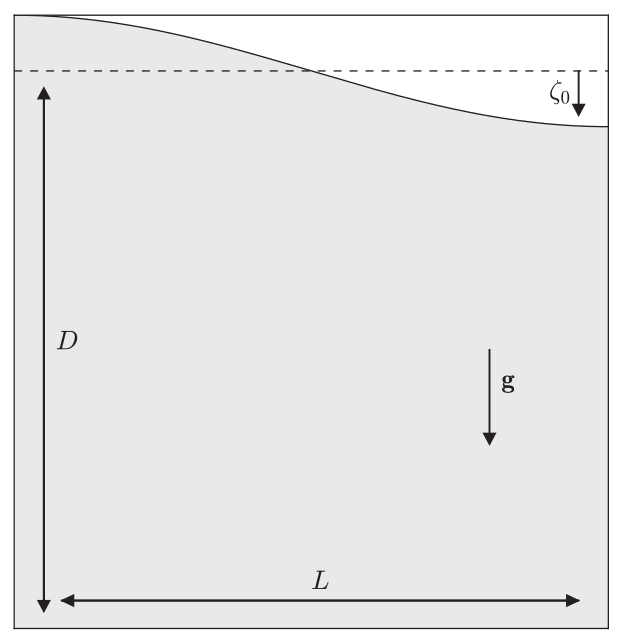
\includegraphics[height=0.8\textwidth]{images/benchmark_relaxation/robh17}\\
{\small Taken from \cite{robh17}. Setup for the free surface relaxation benchmark.
For the tests $\rho=\eta=g=L=D=1$ and $\xi_0=0.005$.}
\end{minipage}\hfill
\begin{minipage}{0.45\textwidth}
\centering
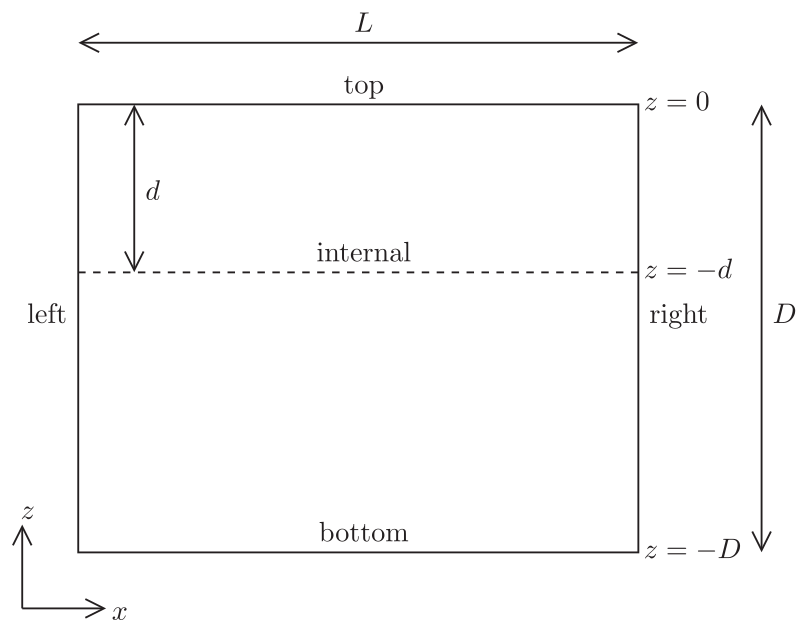
\includegraphics[height=0.8\textwidth]{images/benchmark_relaxation/krwd12}\\
{\small Taken from \cite{krwd12}. $D=3\cdot 10^6$,$\eta=10^{21}$, $\rho=4500$, $g=10$, $\xi_0=10^3$m, and 
$L=D/4,D/2,D,2D,4D$.}
\end{minipage}
\end{center}
and the infinitesimal sinusoidal perturbations to the free surface is given by
\[
\xi(x,t=0)=\xi_0 \cos \left( \frac{2 \pi n x}{L}  \right)
\]
where $n$ is a wavenumber which is an integer multiple of 1/2 (taken to be 1/2 exactly in both cases).


%...............................................................
\subsubsection{the plastic brick}

\Literature \cite{hans03,moml07,lemm08,kaus10,egat10,qurj09,mishin11,maie12,spmw16,gltf18,frbt19,aspectmanual}

Pretty much all of the brick-type (elasto-)visco-plastic experiments in the literature
introduce a weak seed at the bottom of the domain to seed deformation (the shear bands
will ultimately stem from it). 
Dimensioned and dimensionless experiments have been carried out, with or without 
elastic behaviour, with or without adaptive mesh refinement, with first order and 
second order quadrilateral elements or Taylor-Hood triangles, with or without 
Newton algorithm, in extension and compression, with or without time-stepping,
with or without viscous lower layer. 


\begin{center}
\begin{minipage}{0.45\textwidth}
\centering
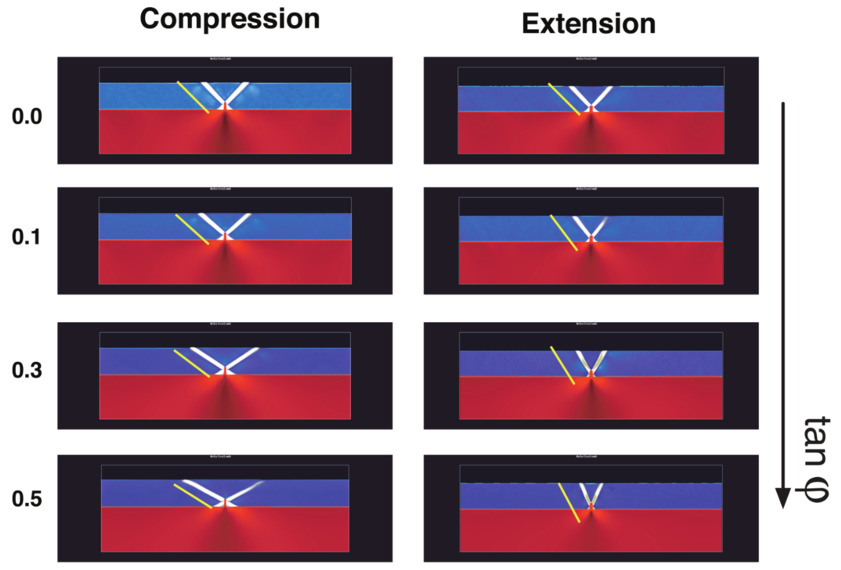
\includegraphics[height=0.8\textwidth]{images/benchmark_brick/moml07}\\
{\small Moresi et al, 2007 \cite{moml07}}
\end{minipage}\hfill
\begin{minipage}{0.45\textwidth}
\centering
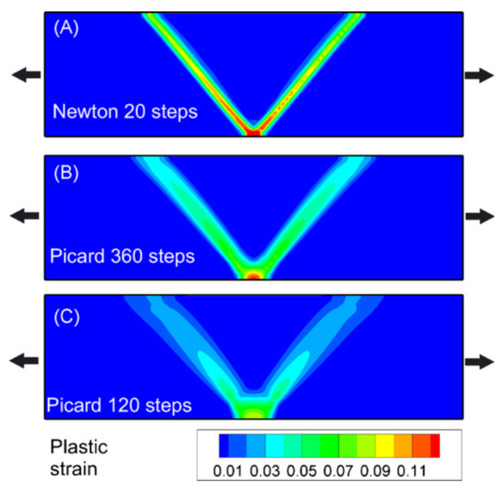
\includegraphics[height=0.8\textwidth]{images/benchmark_brick/poso08}\\
{\small Popov et al, 2008 \cite{poso08}}
\end{minipage}
\end{center}

\begin{center}\noindent\rule{8cm}{0.4pt}\end{center}

\begin{center}
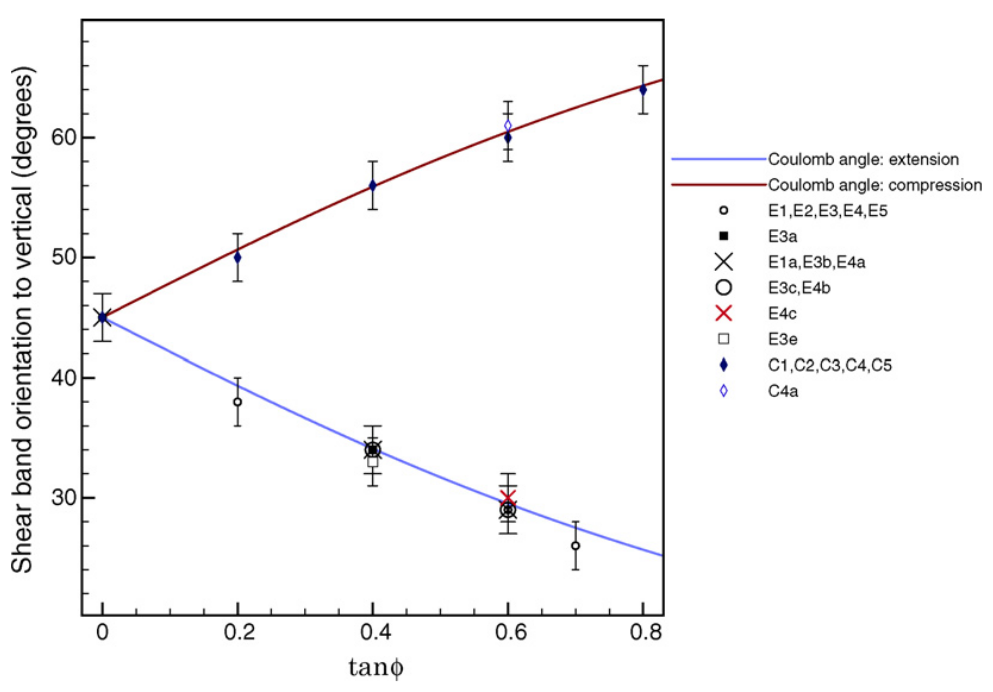
\includegraphics[width=5cm]{images/benchmark_brick/lemm08a}
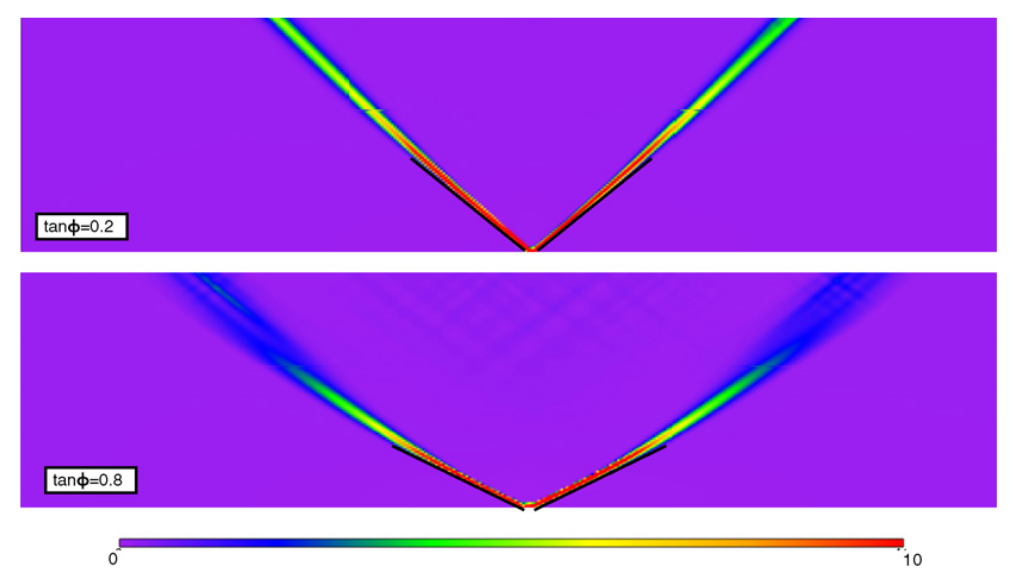
\includegraphics[width=5cm]{images/benchmark_brick/lemm08b}
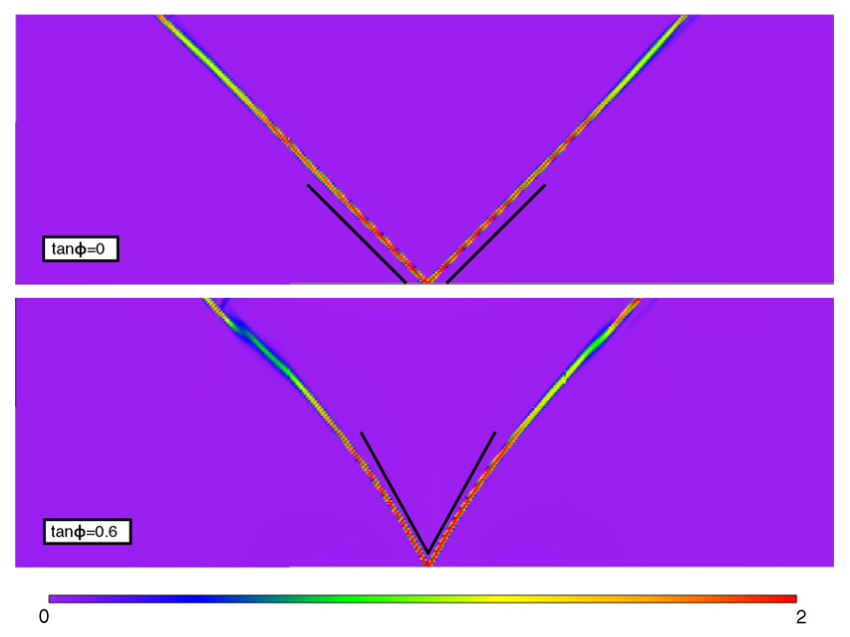
\includegraphics[width=5cm]{images/benchmark_brick/lemm08c}\\
{\small Lemiale et al, 2008 \cite{lemm08}}
\end{center}

\begin{center}\noindent\rule{8cm}{0.4pt}\end{center}

\begin{center}
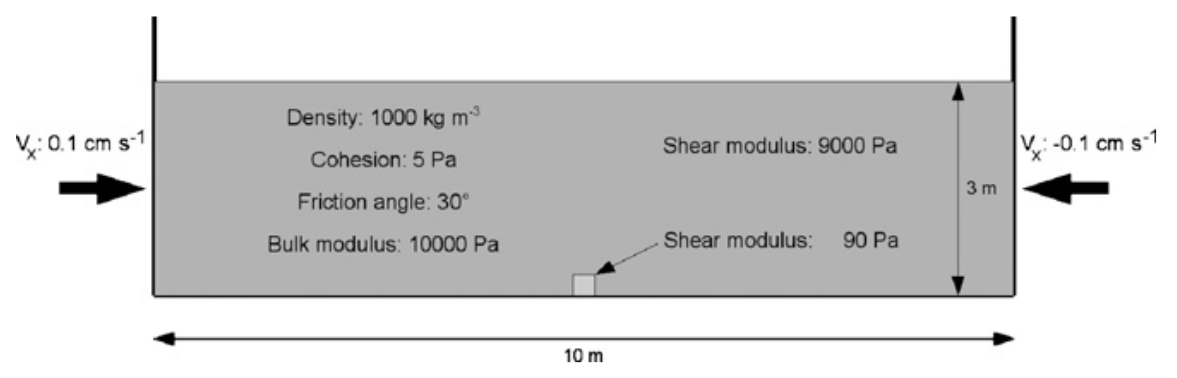
\includegraphics[width=7cm]{images/benchmark_brick/qurj09b}
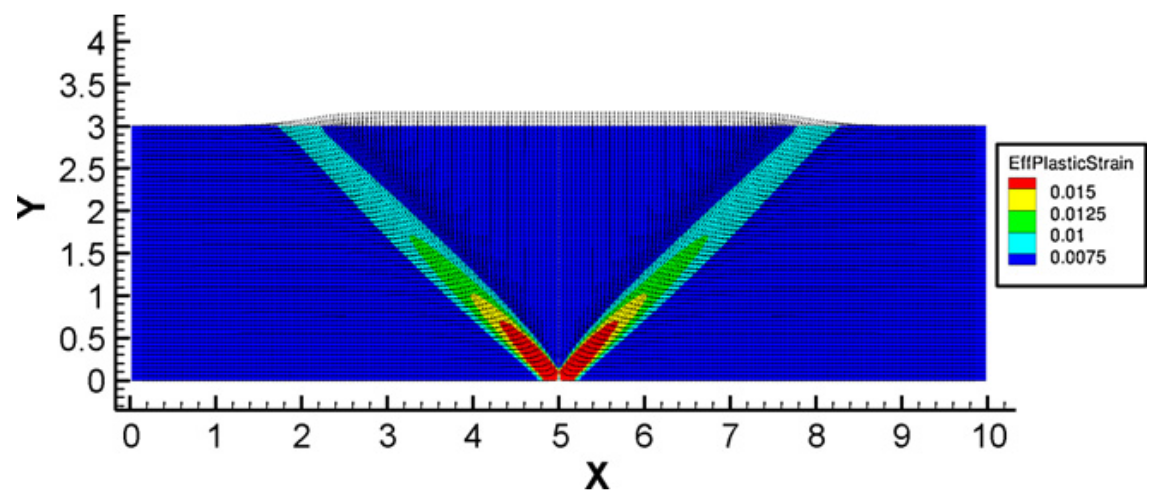
\includegraphics[width=6cm]{images/benchmark_brick/qurj09a}\\
{\small Quinteros et al., 2009 \cite{qurj09}}
\end{center}

\begin{center}\noindent\rule{8cm}{0.4pt}\end{center}

\begin{center}
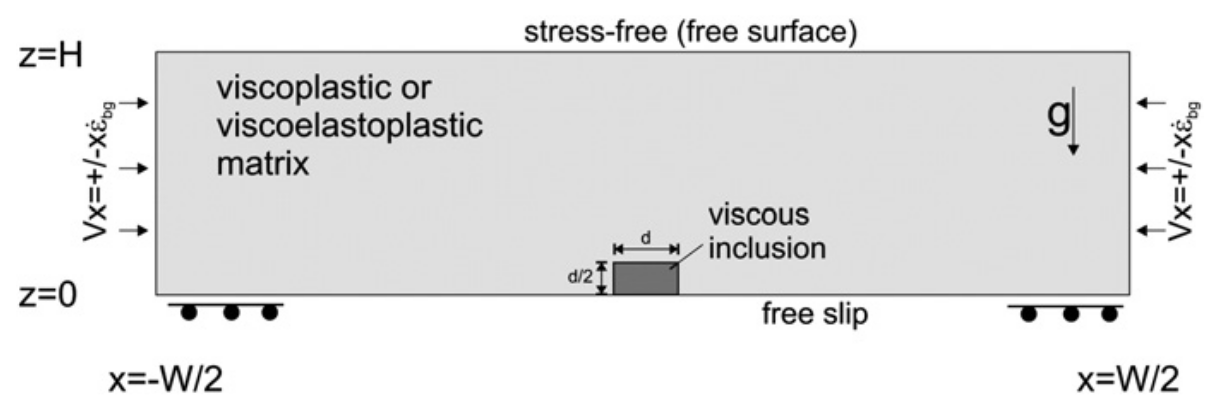
\includegraphics[width=5cm]{images/benchmark_brick/kaus10a}
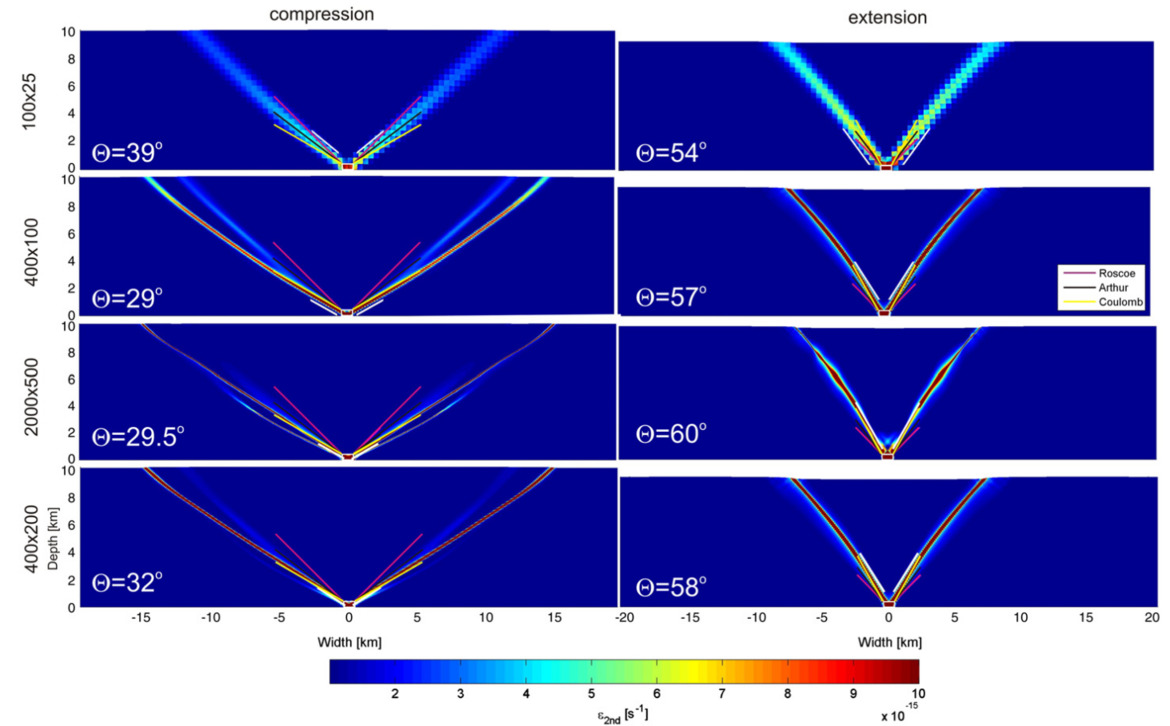
\includegraphics[width=5cm]{images/benchmark_brick/kaus10b}
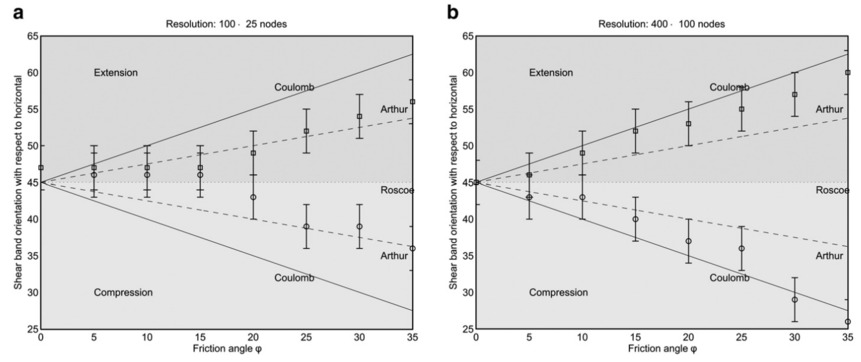
\includegraphics[width=5cm]{images/benchmark_brick/kaus10c}\\
{\small Kaus, 2010 \cite{kaus10}}
\end{center}

\begin{center}\noindent\rule{8cm}{0.4pt}\end{center}

\begin{center}
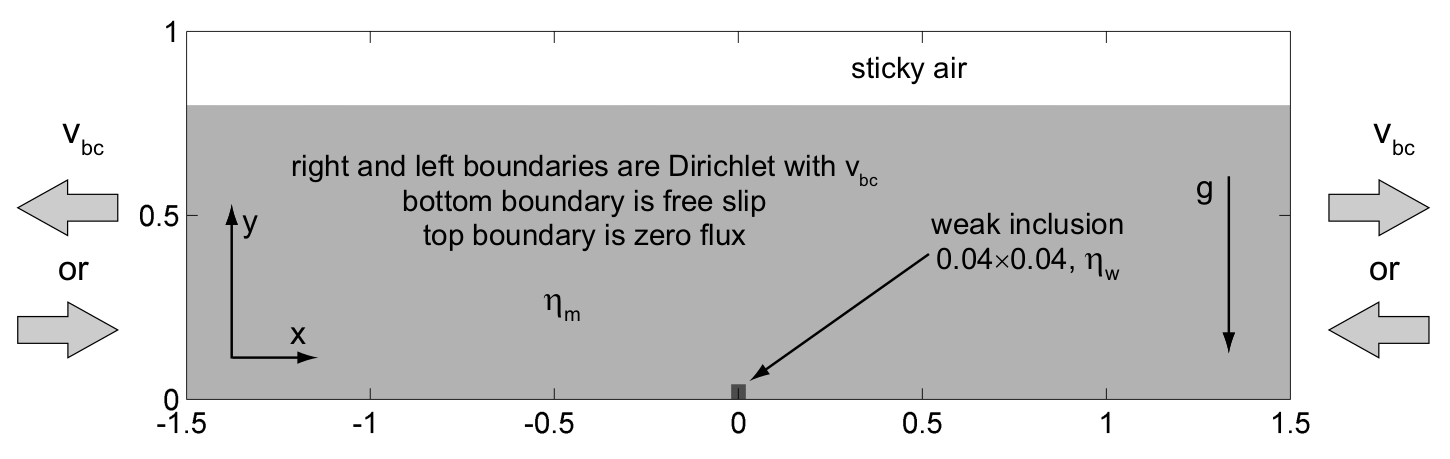
\includegraphics[width=3.74cm]{images/benchmark_brick/mishina}
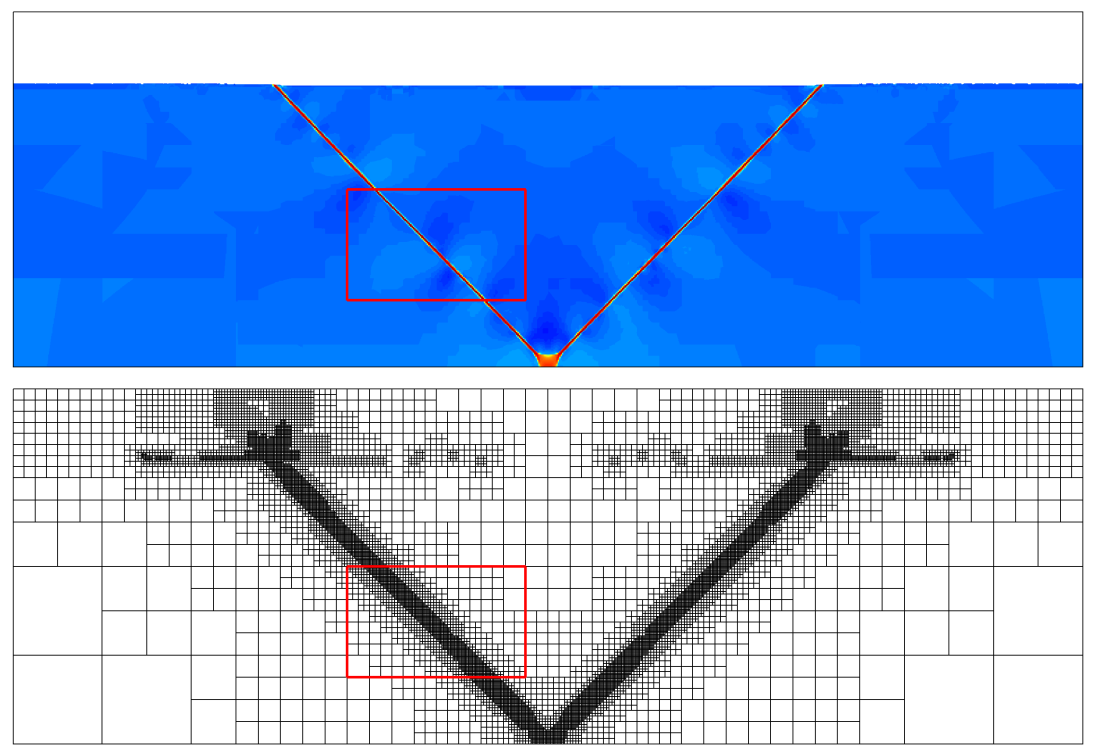
\includegraphics[width=3.74cm]{images/benchmark_brick/mishinb}
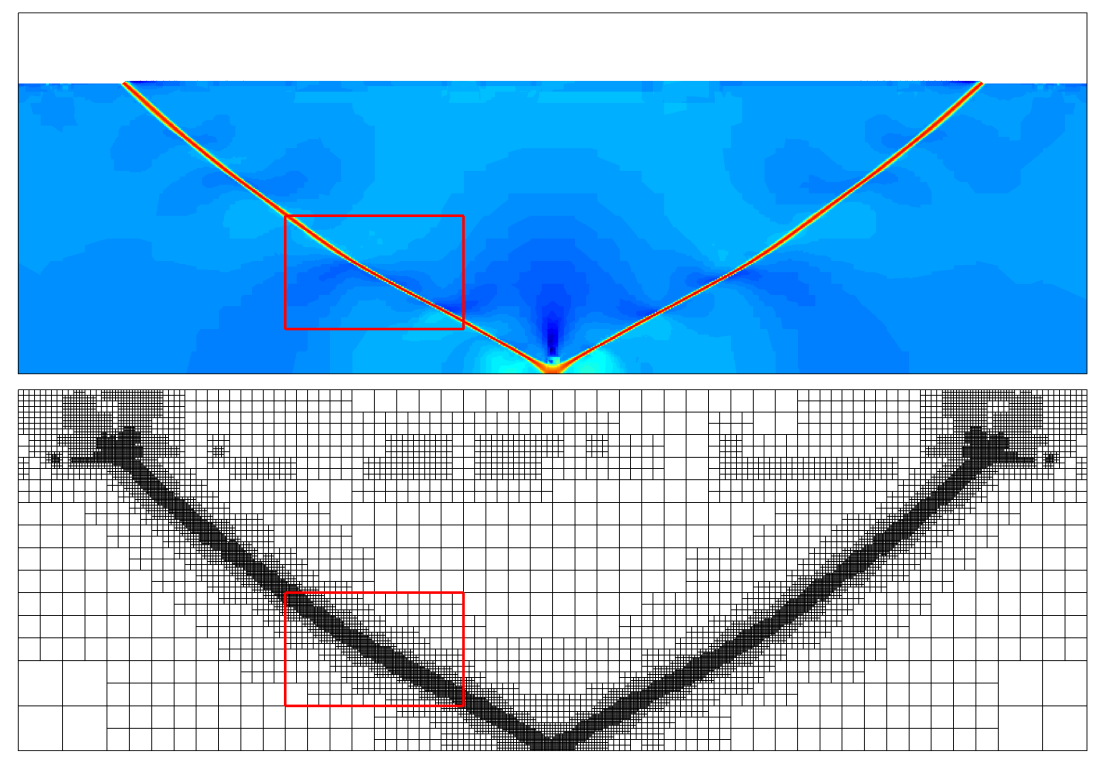
\includegraphics[width=3.74cm]{images/benchmark_brick/mishinc}
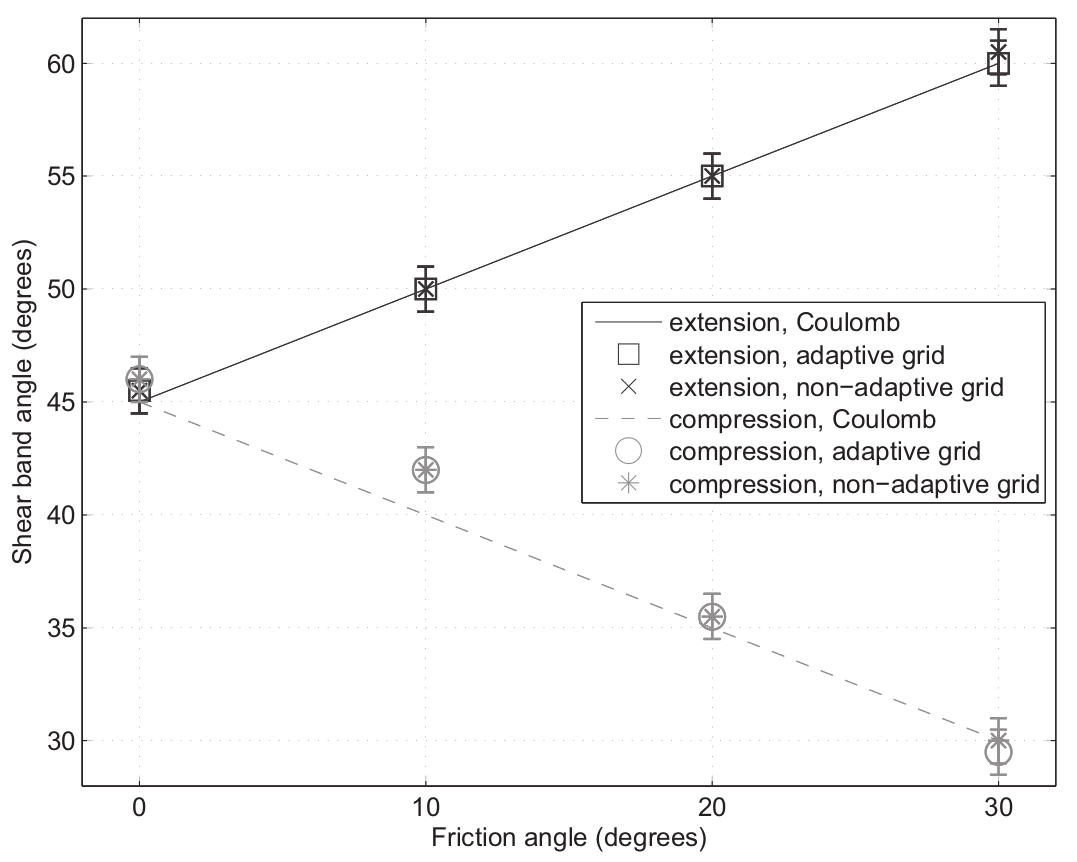
\includegraphics[width=3.74cm]{images/benchmark_brick/mishind}\\
{\small Mishin, phd thesis, 2011 \cite{mishin11}}
\end{center}

\begin{center}\noindent\rule{8cm}{0.4pt}\end{center}

\begin{center}
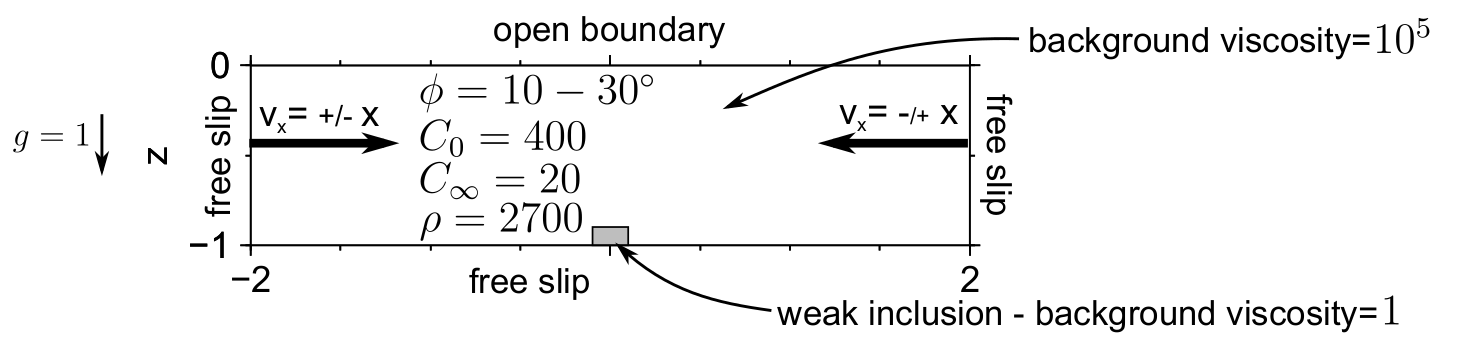
\includegraphics[width=8cm]{images/benchmark_brick/maie12a}
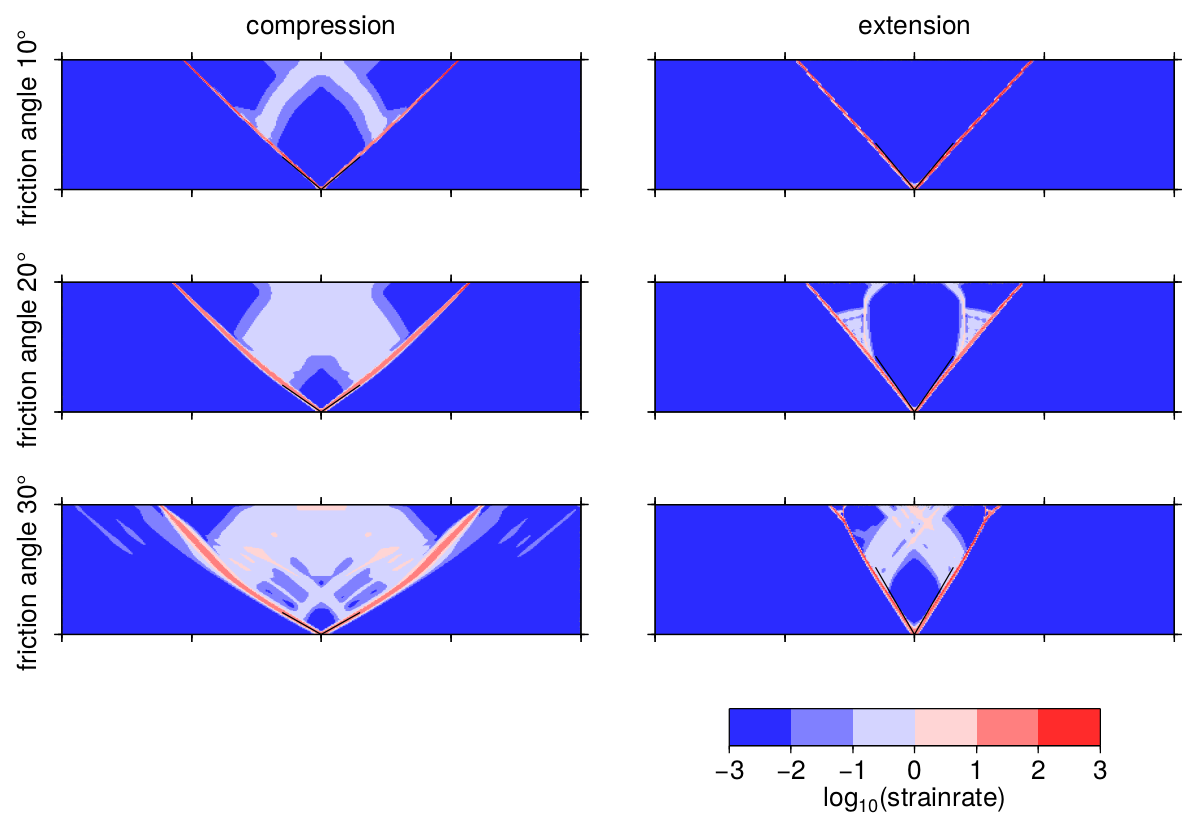
\includegraphics[width=5cm]{images/benchmark_brick/maie12b}\\
{\small Maierova, phd thesis, 2012 \cite{maie12}}
\end{center}

\begin{center}\noindent\rule{8cm}{0.4pt}\end{center}

\begin{center}
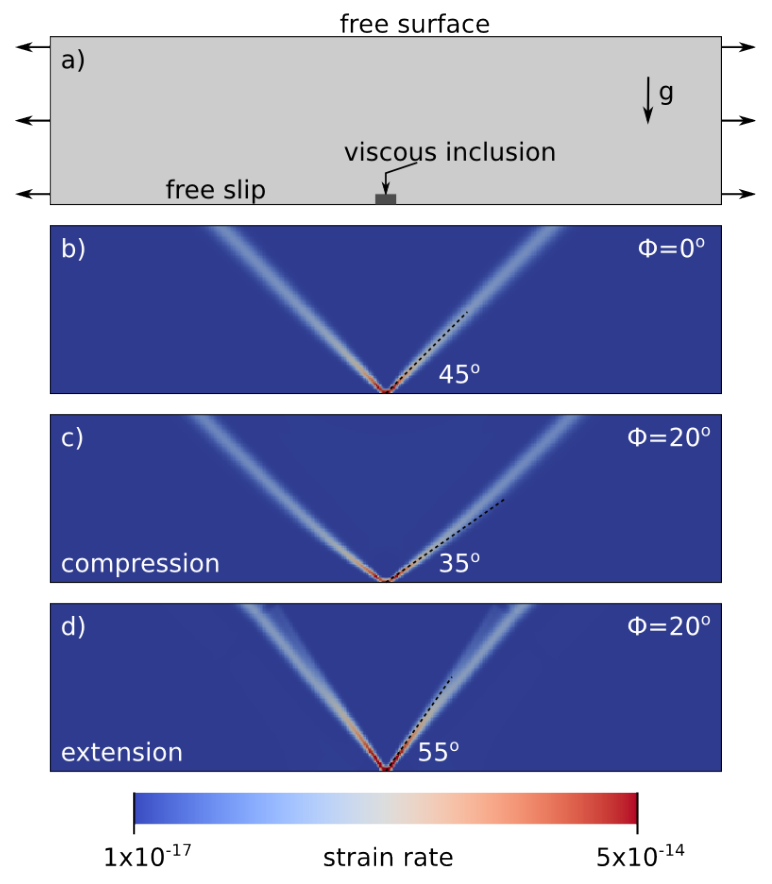
\includegraphics[width=5cm]{images/benchmark_brick/thie14a}
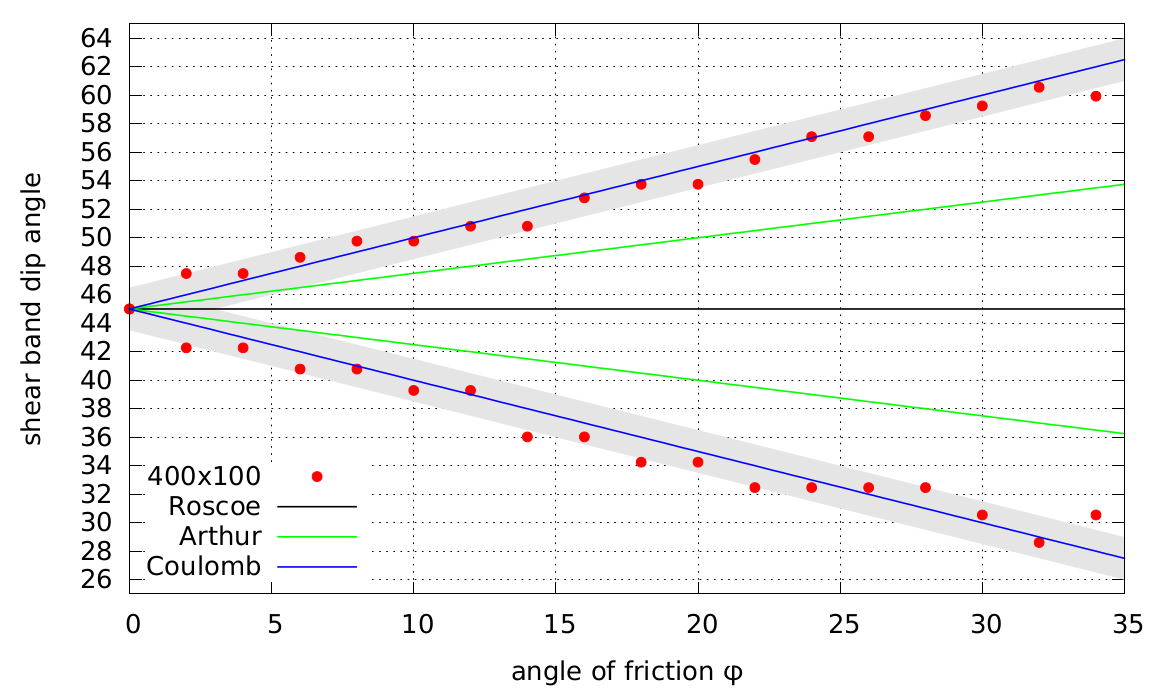
\includegraphics[width=8cm]{images/benchmark_brick/thie14b}\\
{\small Thieulot, 2014 \cite{thie14}}
\end{center}

\begin{center}\noindent\rule{8cm}{0.4pt}\end{center}

\begin{center}
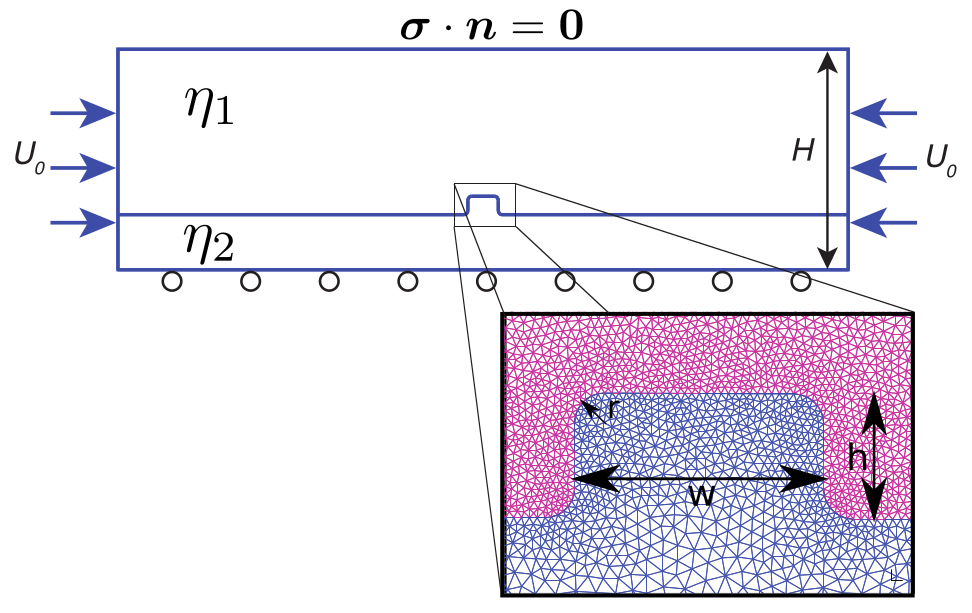
\includegraphics[width=5cm]{images/benchmark_brick/spmw16a}
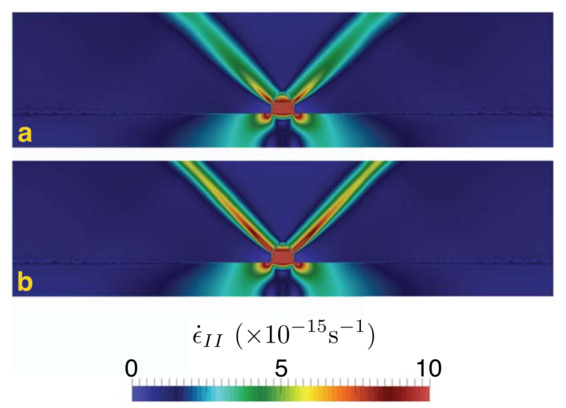
\includegraphics[width=5cm]{images/benchmark_brick/spmw16b}\\
{\small Spiegelman et al, 2016 \cite{spmw16}}
\end{center}

\begin{center}\noindent\rule{8cm}{0.4pt}\end{center}

\begin{center}
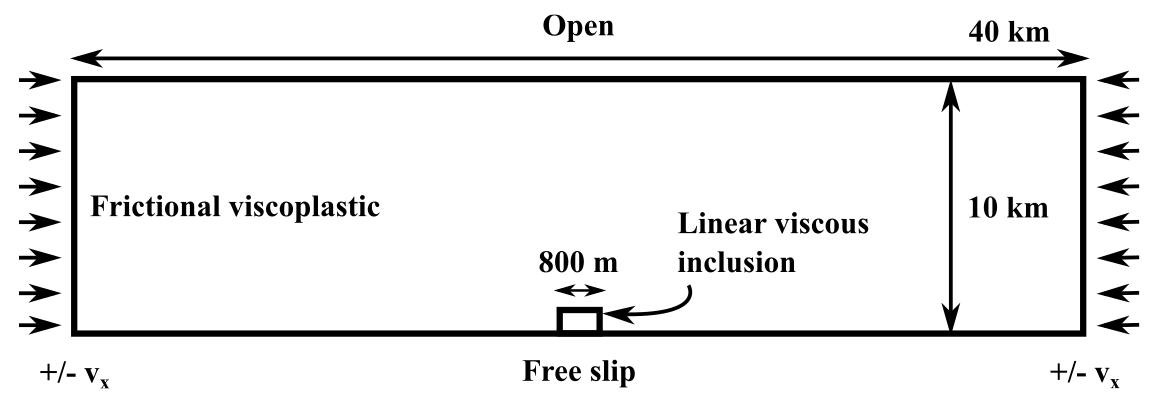
\includegraphics[width=5cm]{images/benchmark_brick/gltf18a}
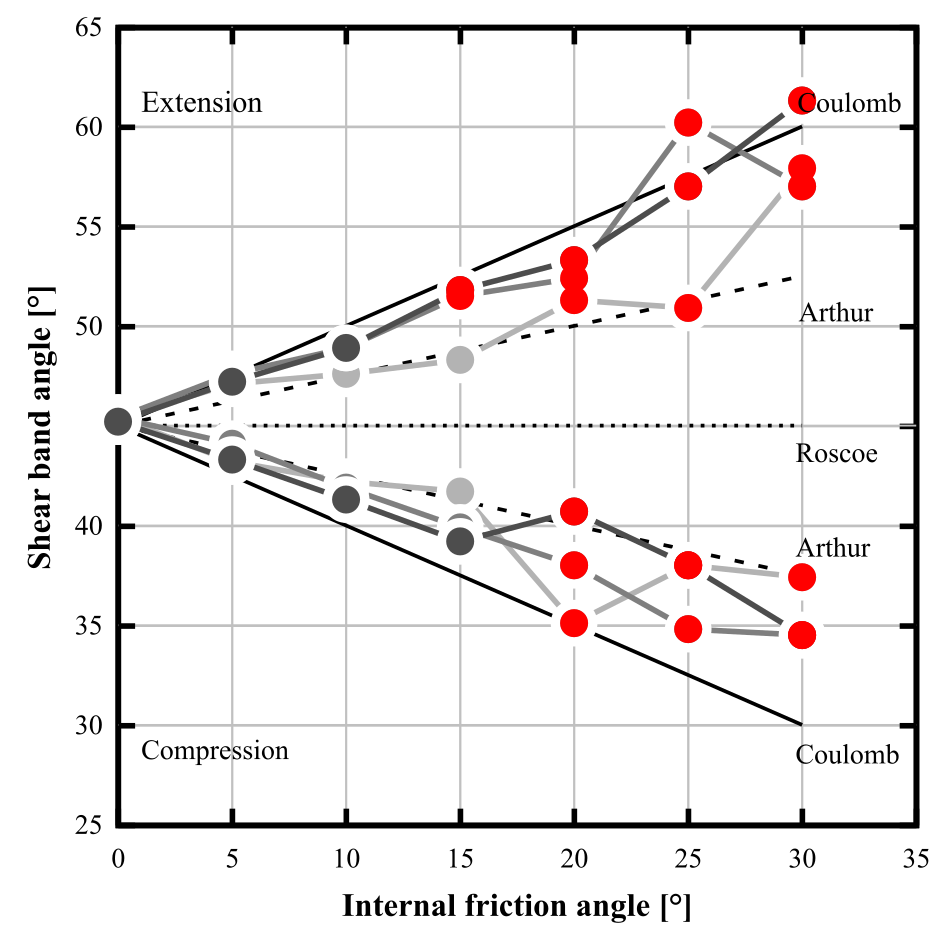
\includegraphics[width=5cm]{images/benchmark_brick/gltf18b}
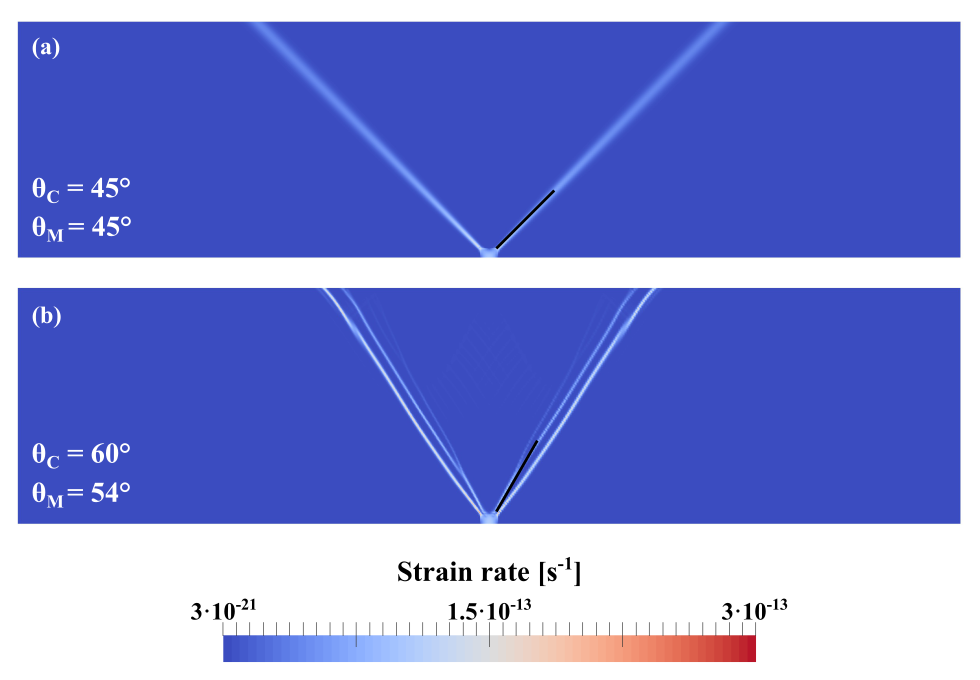
\includegraphics[width=5cm]{images/benchmark_brick/gltf18c}\\
{\small Glerum et al, 2018 \cite{gltf18}}
\end{center}

\begin{center}\noindent\rule{8cm}{0.4pt}\end{center}

\begin{center}
\begin{minipage}{0.45\textwidth}
\centering
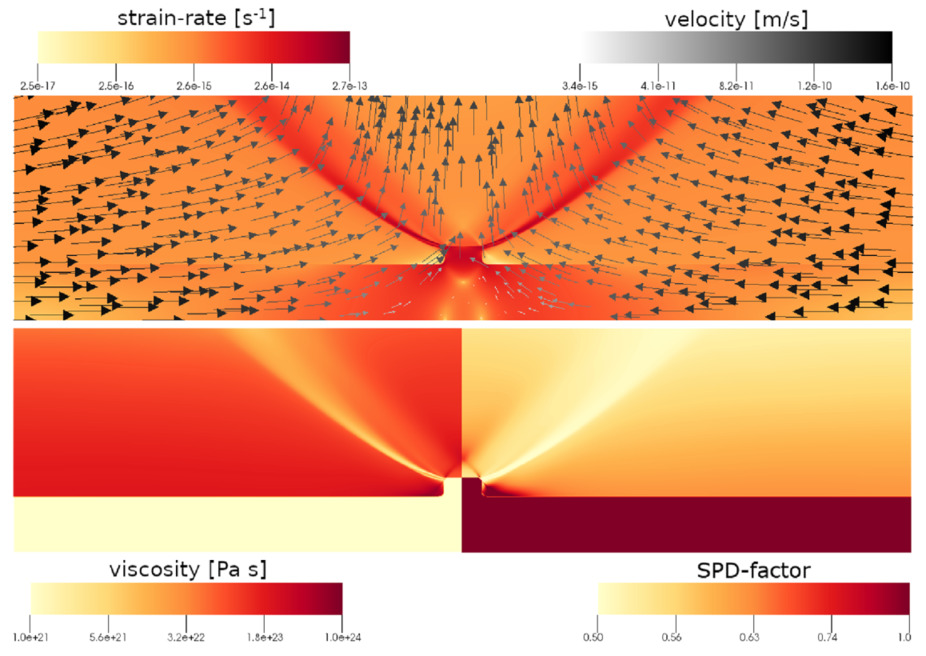
\includegraphics[height=0.8\textwidth]{images/benchmark_brick/frbt19}\\
{\small Fraters et al, 2019 \cite{frbt19}}
\end{minipage}\hfill
\begin{minipage}{0.45\textwidth}
\centering
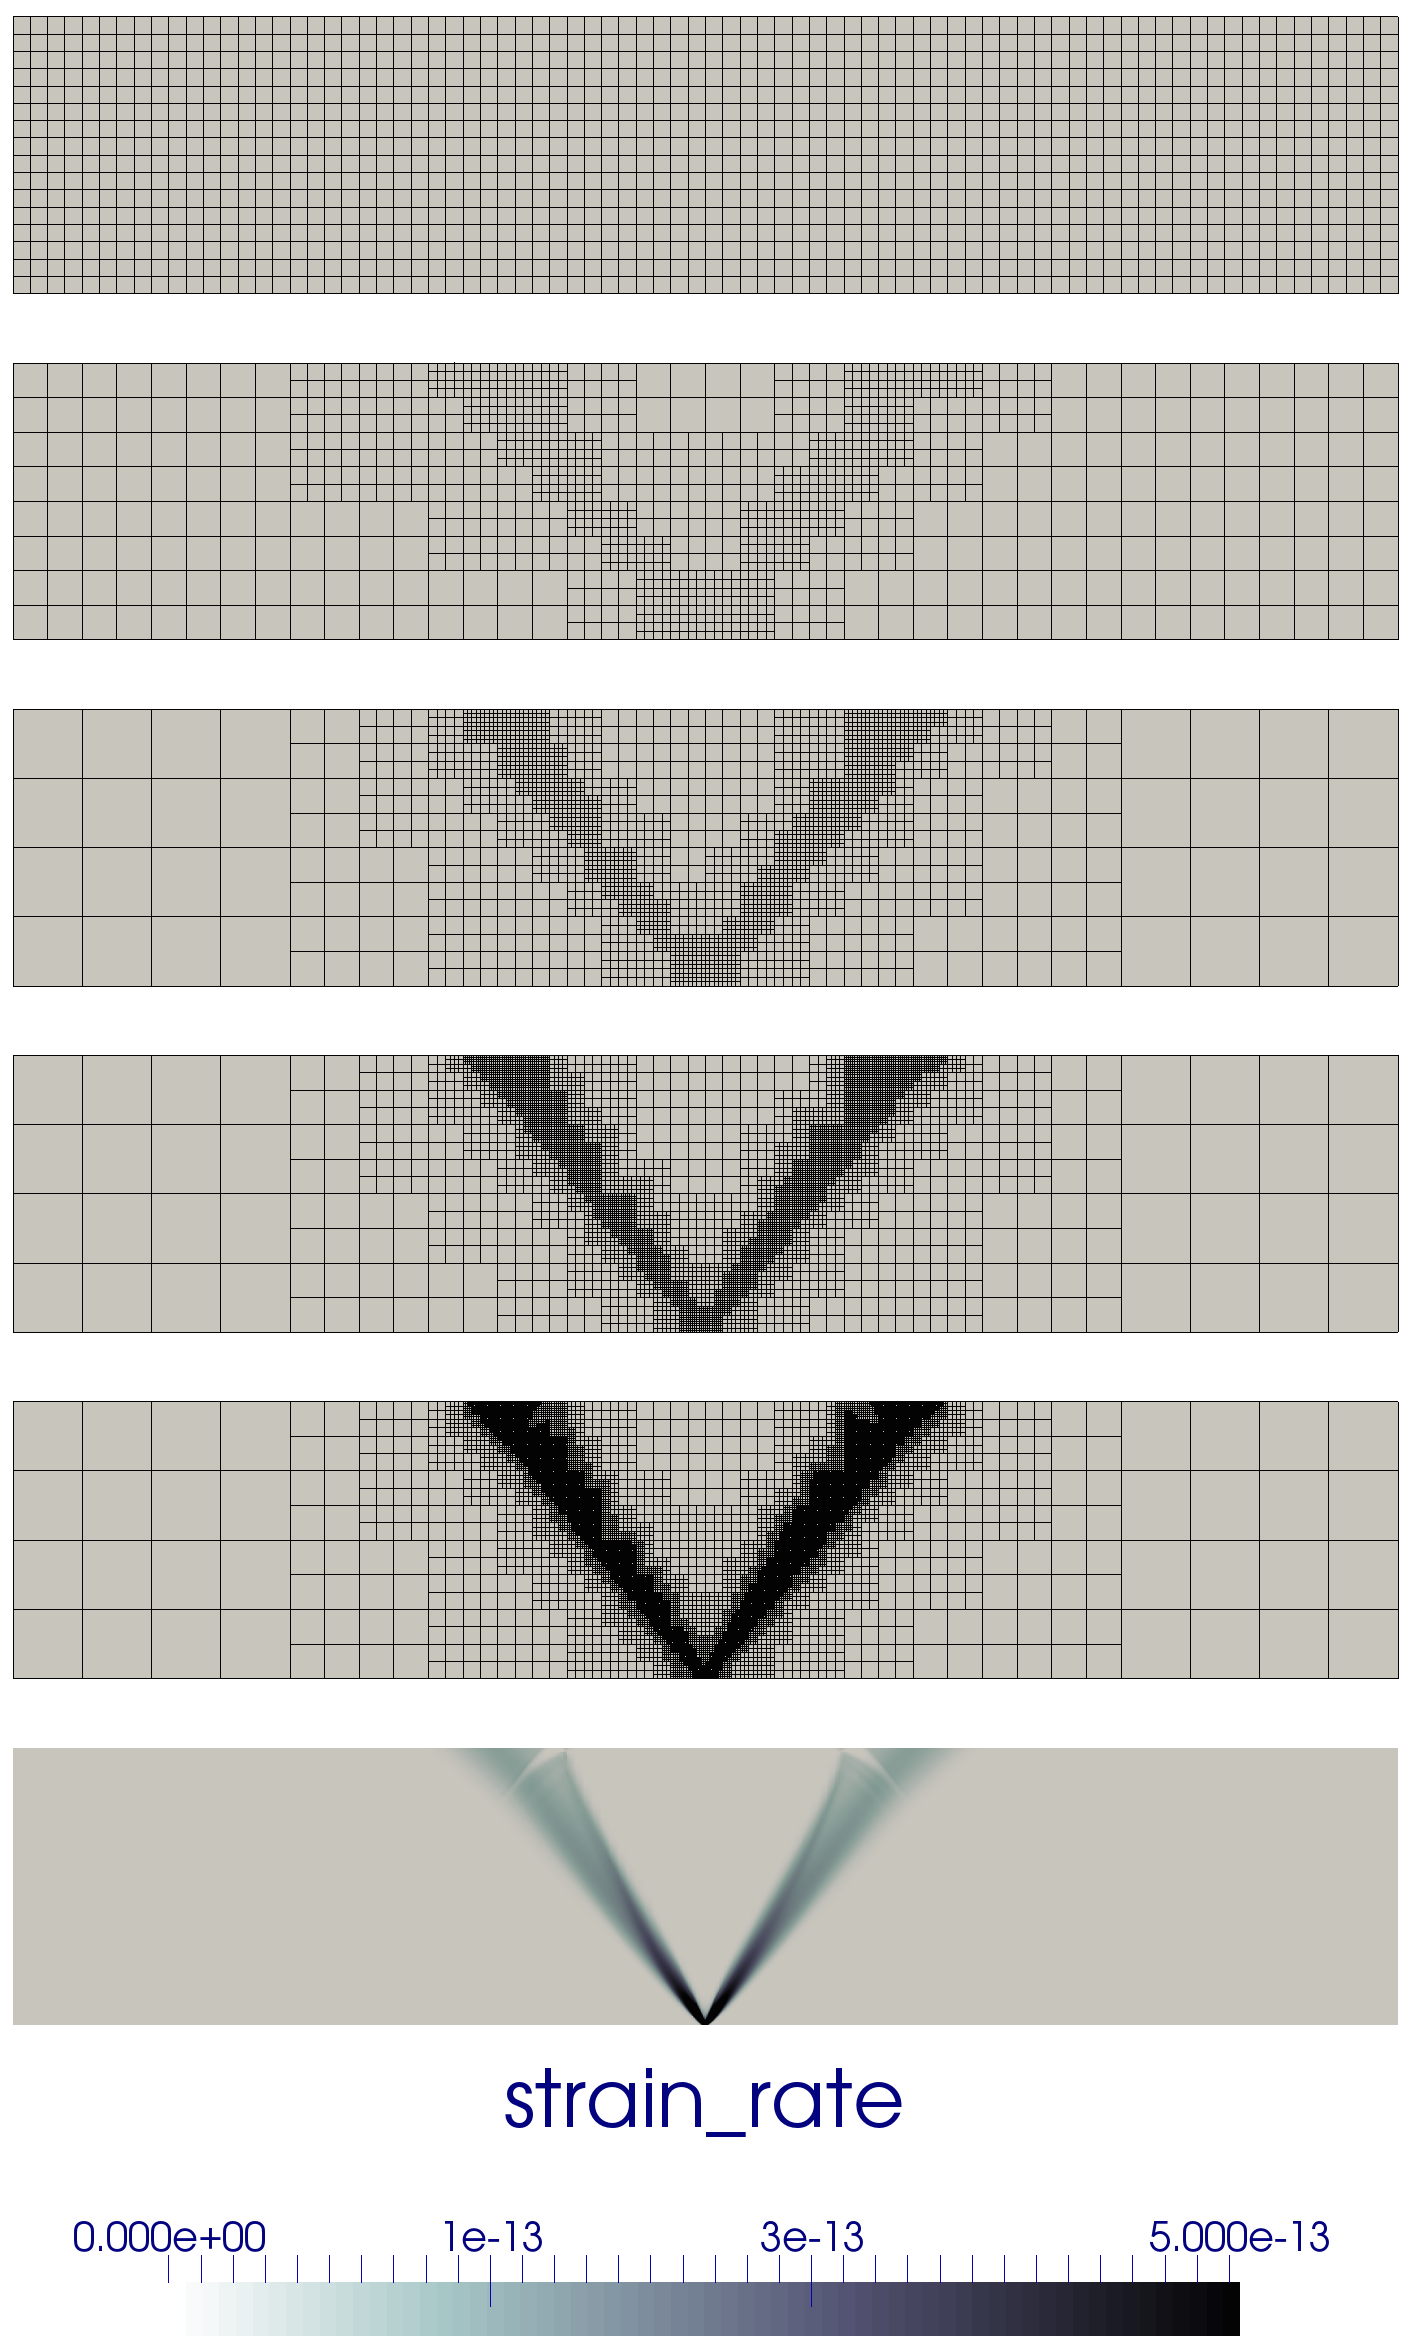
\includegraphics[height=0.8\textwidth]{images/benchmark_brick/aspectmanual}\\
{\small Aspect manual \cite{aspectmanual}}
\end{minipage}
\end{center}

%..........................................................................
\subsubsection{Infinite plate with a circular hole \cite{rama16}}
\mscthesis \index{MSc Thesis}

An infinite plate with a circular hole of radius $a$ 
is subjected to a unidirectional tensile load of $\sigma$ in the $x$ direction as shown
in the figure. In this case, only one quarter of the domain is analysed due
to symmetry along $x$ and $y$ axis. 

\begin{center}
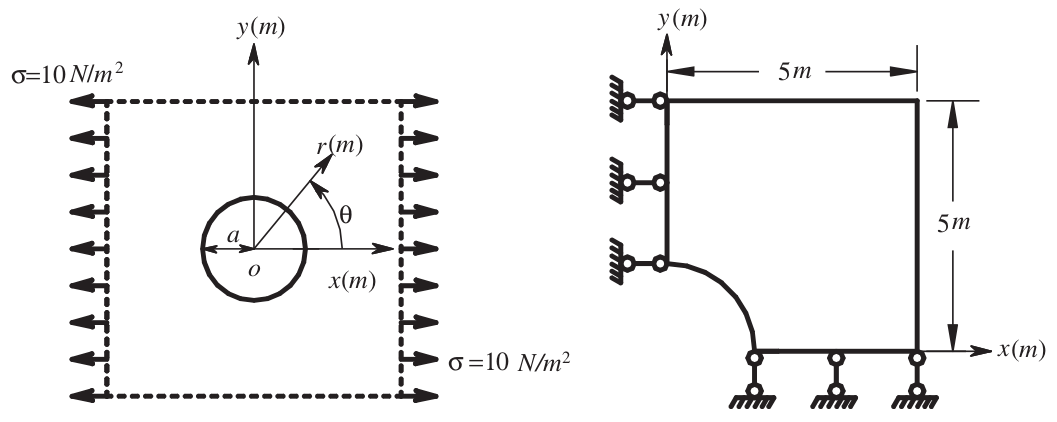
\includegraphics[width=0.65\textwidth]{images/benchmark_hole/yobu02}
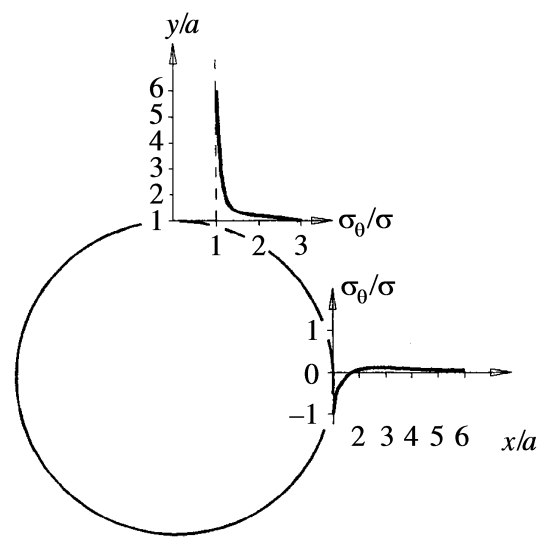
\includegraphics[width=0.25\textwidth]{images/benchmark_hole/yobu02b}\\
{\scriptsize Left: An infinite plate with a circular hole subjected to unidirectional tension 
and its quarter model with symmetric conditions imposed on the left and bottom edges.
Right: Tangential stress distribution for $\theta=0$  and $\theta=\pi/2$. \cite{yobu02}}
\end{center}

The inner boundary of the hole is traction free and the right edge was
imposed with the tractions based on the analytical solutions.
The left edge is constrained in the $x$ direction and the bottom
edge is constrained in the $y$ direction, respectively. The plane stress
condition is considered and the parameters are: 
Young modulus $E=$3e7 MPa, Poisson Ratio $\nu=$0.3, Load $\sigma$=10 N/m$^2$, a=1m.

The analytical stress components for this
problem are 

\begin{eqnarray}
\sigma_{xx}(x,y) &=& \sigma \left(  1-\frac{a^2}{r^2}\left(\frac{3}{2}\cos 2\theta + \cos 4\theta \right) 
+ \frac{3a^4}{2r^4} \cos 4\theta \right) \\
\sigma_{yy}(x,y) &=& -\sigma \left( \frac{a^2}{r^2} \left(\frac{1}{2}\cos 2\theta - \cos 4\theta \right) 
- \frac{3a^4}{2r^4} \cos 4\theta \right) \\
\sigma_{xy}(x,y) &=& -\sigma \left( \frac{a^2}{r^2} \left(\frac{1}{2}\sin 2\theta + \sin 4\theta\right) 
+ \frac{3a^4}{2r^4} \sin 4\theta \right) 
\end{eqnarray}

Note that \cite{rama16} cites \cite{chnn10} which cites the book \cite[p772]{yobu02} 
which cites \cite{budynas} for the solution!
\todo[inline]{there are discrepancies between \cite{rama16} and \cite{chnn10}}

Following \cite{yobu02}, it can be shown, from linear elasticity, that the tangential
stress throughout the plate is given by
\[
\sigma_\theta = \frac{\sigma}{2} \left[ 1+\frac{a^2}{r^2} - \left( 1+3\frac{a^4}{r^4}  \right) \cos 2\theta   \right]
\]
The maximum stress is $\sigma_\theta=3\sigma$ at $r=a$ and $\theta=\pm \pi/2$. Along the surface of the hole, 
the tangential stress is $-\sigma$ at y $\theta=0$  and $\theta=\pi$, 
and increases, as $\theta$ increases, to $3\sigma$ at $\theta=\pi/2$ and $\theta=3\pi/2$.
 

%..............................................................................
\subsubsection{Slope stability for elasto-plastic materials a la \cite{rama16}}
\mscthesis \index{MSc Thesis}

The bottom of the domain is constrained and the model is 
subjected to gravitational load. The material properties considered are

Young modulus 20e3 MPa, Poisson Ratio 0.49, Constitutive law Mohr-Coulomb 
(friction angle $\phi=20$\degree, 
dilatancy angle $\phi=20$\degree, cohesion $c$=50Mpa).

\begin{center}
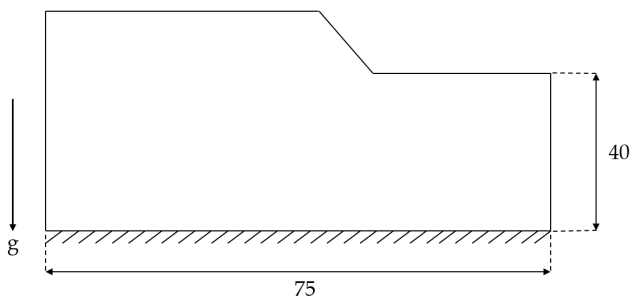
\includegraphics[width=0.5\textwidth]{images/benchmark_slope/rama16c}
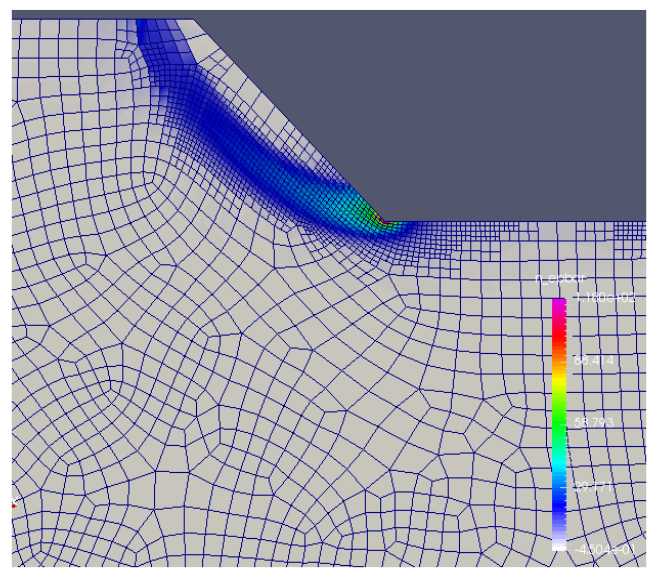
\includegraphics[width=0.4\textwidth]{images/benchmark_slope/rama16b}\\
{\scriptsize Left: Slope stability problem setup; Right: Adaptive Refinement based 
on Plasticity Indicator}
\end{center}


%..............................................................................
\subsubsection{Time-dependent benchmark in an annulus}\label{sec:tdba}

This benchmark is presented in Gass{m\"o}ller et al \cite{galb19}.
The domain is a 2D annulus with inner and outer radii $R_1=1$ and $R_2=2$, respectively.
In this situation, the incompressible isothermal Stokes equations and their solution
can be expressed in a cylindrical coordinate system in terms of the radius $r$ and the
azimuthal angle $\theta$. The viscosity is set to $eta=1$, and the density is given by
\begin{equation}
\rho(r,\theta)=48r^5
\end{equation}
The gravity vector is set to 
\begin{equation}
\vec{g}(r,\theta)=\frac{r^3}{384} \vec{e}_r + \vec{e}_\theta
\end{equation}
Note that this gravity vector is not the gradient of a gravity potential
and consequently not physical.
The Stokes system can then be solved using a separation of variables
approach and yields
\begin{equation}
\vec{\upnu}=-r^7 \vec{e}_\theta
\quad\quad
p(r,\theta)=\frac{r^9}{72}-\frac{512}{72}
\end{equation}
\begin{center}
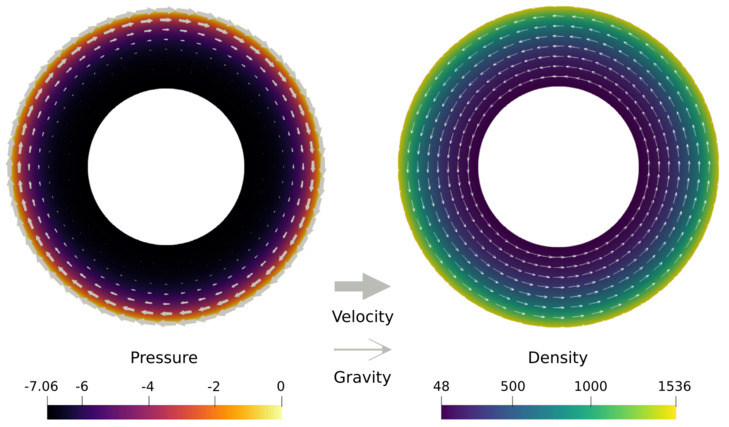
\includegraphics[width=12cm]{images/benchmark_annulus/galb19}\\
{\scriptsize Taken from \cite{galb19}}
\end{center}
Rather importantly, this benchmark was arrived at by means of a stream function (see Section~\ref{sec:streamfunction}) 
$\psi(r,\theta)=F(r)G(\theta)$ with $F(r)=r^8/8$ and $G(\theta)=1$.

%..............................................................................
\subsubsection{Convection in 2D-box} \label{sec:citb}

We start from the following stream function (see Section~\ref{sec:streamfunction}):
\begin{equation}
\psi(x,y)=\frac{1}{\pi} \sin \pi x \sin \pi y
\end{equation}
which yields:
\begin{eqnarray}
u(x,y)&=&\frac{\partial \psi}{\partial y} = \sin \pi x \cos \pi y \nn\\
v(x,y)&=&-\frac{\partial \psi}{\partial x} = - \cos \pi x \sin \pi y
\end{eqnarray}
The pressure field is 
\begin{equation}
p(x,y) = 2\pi \cos (\pi x) \cos (\pi y) 
\end{equation}
with 
\begin{equation}
\rho(x,y)=\sin(\pi x) \sin (\pi y)
\qquad\qquad
g_y = -4\pi ^2 \frac{\cos (\pi x)}{\sin (\pi x)}
\end{equation}

\begin{center}
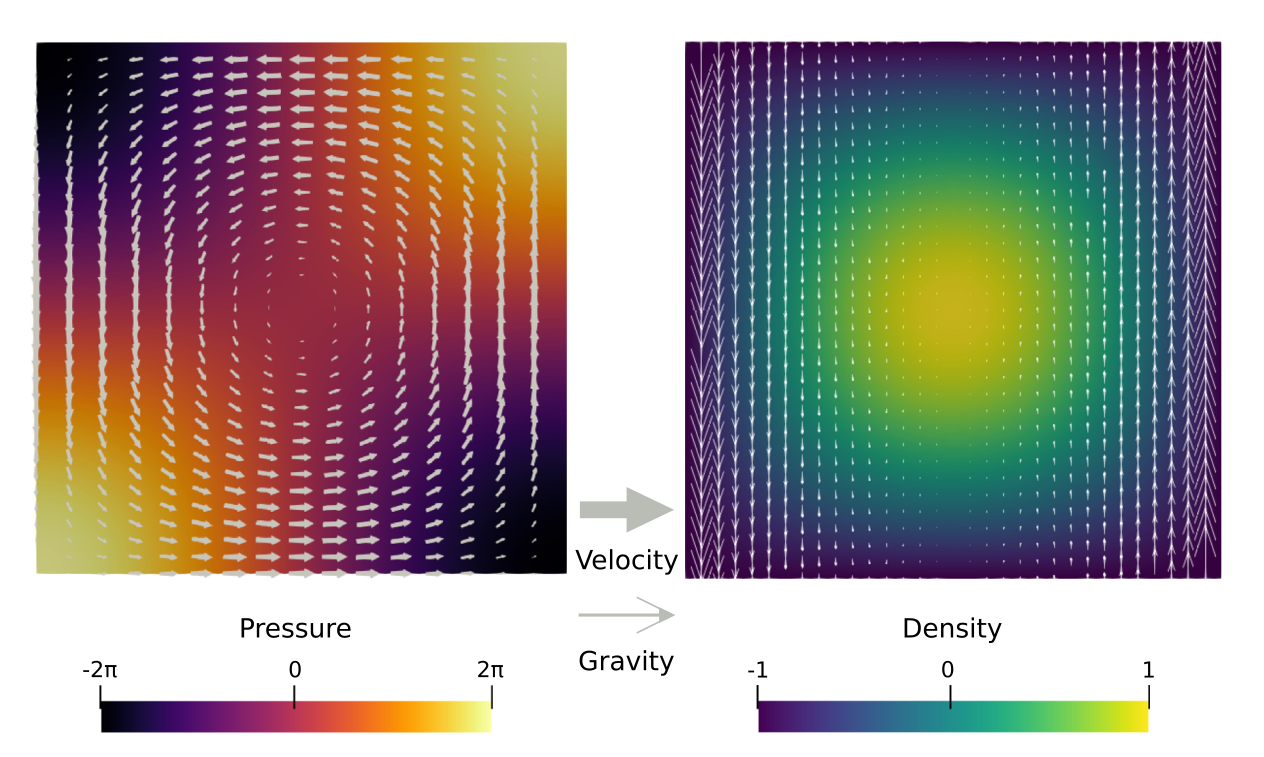
\includegraphics[width=12cm]{images/benchmark_convbox/galb19}\\
{\scriptsize Taken from \cite{galb19}}
\end{center}

\begin{eqnarray}
v_{rms} 
&=& \sqrt{\frac{1}{L_xL_y} \int_0^1 \int_0^1 (u^2+v^2) dxdy} \nn\\
&=& \sqrt{\int_0^1 \int_0^1 ( \sin^2 (\pi x) \cos^2 (\pi y) + \cos^2 (\pi x) \sin^2 (\pi y) ) dxdy} \nn\\
&=& \sqrt{ \int_0^1 \sin^2 (\pi x) dx  \cdot \int_0^1 \cos^2 (\pi y) dy + \int_0^1 \cos^2 (\pi x) dx \cdot \int \sin^2 (\pi y) dy } \nn\\
&=& \sqrt{\frac{1}{2} \frac{1}{2}+ \frac{1}{2} \frac{1}{2} }\nn\\
&=& \frac{\sqrt{2}}{2} \nn\\
&\simeq& 0.70711...
\end{eqnarray}


%..............................................................................
\subsubsection{The sinker problem}\label{sec:sinker}

This experiment is not a benchmark stricto sensu since there is no analytical solution. However, it is widely used in the technical literature because of its simple setup and since it allows to test solving strategies.
Also, it can conveniently be carried out in both two and three dimensions.

\paragraph{In two dimensions} The time dependent version of the experiment is for instance to be found 
in Gerya \cite{gery10} and the same is repeated in Thieulot \cite{thie11}.

This simple benchmark provides challenging numerical experiments 
dealing with large viscosity variations within the simulation
domain. It consists of a bulk of fluid 1 ($\eta_1,\rho_1$) 
in which a block of fluid 2 ($\eta_2,\rho_2$) falls under its own
weight. The domain is a square of size $L_x = L_y = 500$ km and the
block is initially centred at point ($x$ = 250 km, $y$ = 400 km) with size
$100 \times 100$ km.
Free slip boundary conditions are imposed on all sides of the domain. 
In \cite{thie11} five experiments have been conducted:
$\eta_1 = 10^{20}$ Pa.s, $\rho_2$ = 3220 kg/m$^3$ ;
$\eta_1 = 10^{21}$ Pa.s, $\rho_2$ = 3300 kg/m$^3$ ;
$\eta_1 = 10^{22}$ Pa.s, $\rho_2$ = 6600 kg/m$^3$ ;
$\eta_1 = 10^{23}$ Pa.s, $\rho_2$ = 3300 kg/m$^3$ ;
$\eta_1 = 10^{24}$ Pa.s, $\rho_2$ = 9900 kg/m$^3$,
while in all experiments the density of the surrounding fluid is
$\rho_1=3200$ kg/m$^3$ and the viscosity of the block is varied between
$10^{19}$ and $5\cdot10^{27}$ Pa.s.

\begin{center}
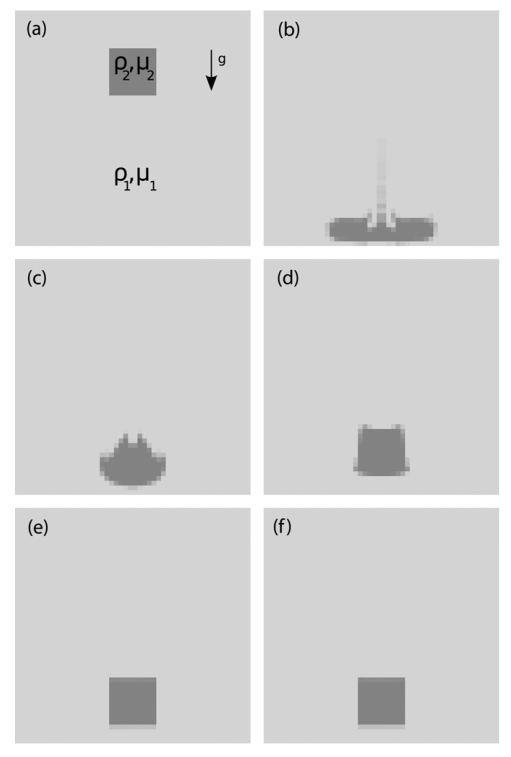
\includegraphics[width=5cm]{images/benchmark_sinker/thie11a}
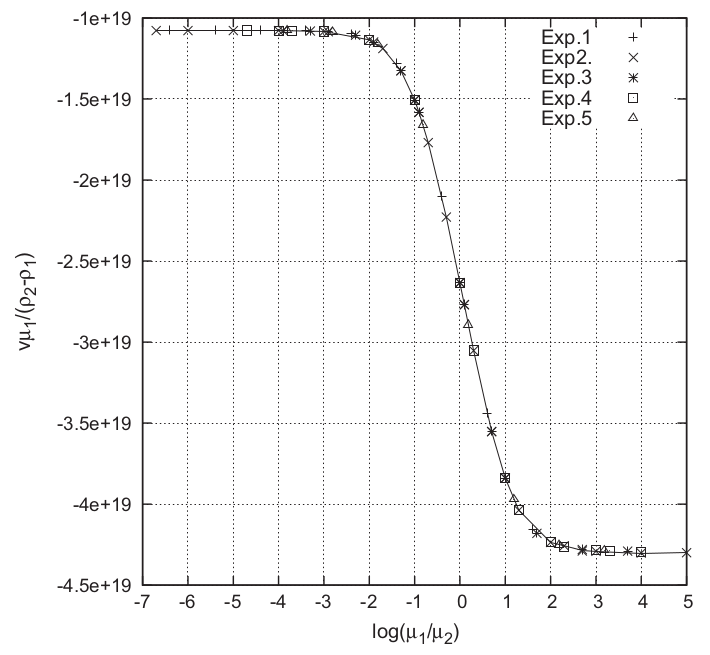
\includegraphics[width=7cm]{images/benchmark_sinker/thie11b}\\
{\scriptsize Left: 
$\eta_1 = 10^{21}$ Pa.s, $\rho_2= 3300$ kg/m$^3$. 
(a) Initial setup; 
(b) $\eta_1 = 10^{21}$ Pa.s at time $t$ = 10 Myrs; 
(c) $\eta_1 = 10^{22}$ Pa.s at time $t$ = 20 Myrs; 
(d) $\eta_1 = 10^{23}$ Pa.s at time $t$ = 20 Myrs; 
(e) $\eta_1 = 10^{25}$ Pa.s at time $t$ = 20 Myrs; 
(f) $\eta_1 = 10^{27}$ Pa.s at time $t$ = 20 Myrs. 
Right: Velocity measurements as a function of the viscosity contrast between
surrounding medium and block for all experiments.
Taken from \cite{thie11}}
\end{center}

\paragraph{In three dimensions}
Let us look at the sinker experiment from Furuichi et al \cite{fumt11}: 
The domain is the unit box the origin at the center of the box. A cube with a viscosity $\eta_1=\Delta \eta$ 
and density $\rho_1 = 1$ was placed at the middle of the domain defined by
$-0.15 \leq x,y,z \leq 0.15$.
The material surrounding the cube has the properties $\eta_0=1$ and $\rho_0 = 0$. 
The body force of the momentum equation was taken as $(0, 0,-\rho g)$ with $g = 1$.
Along all walls on the domain, free-slip boundary conditions were employed.

\begin{center}
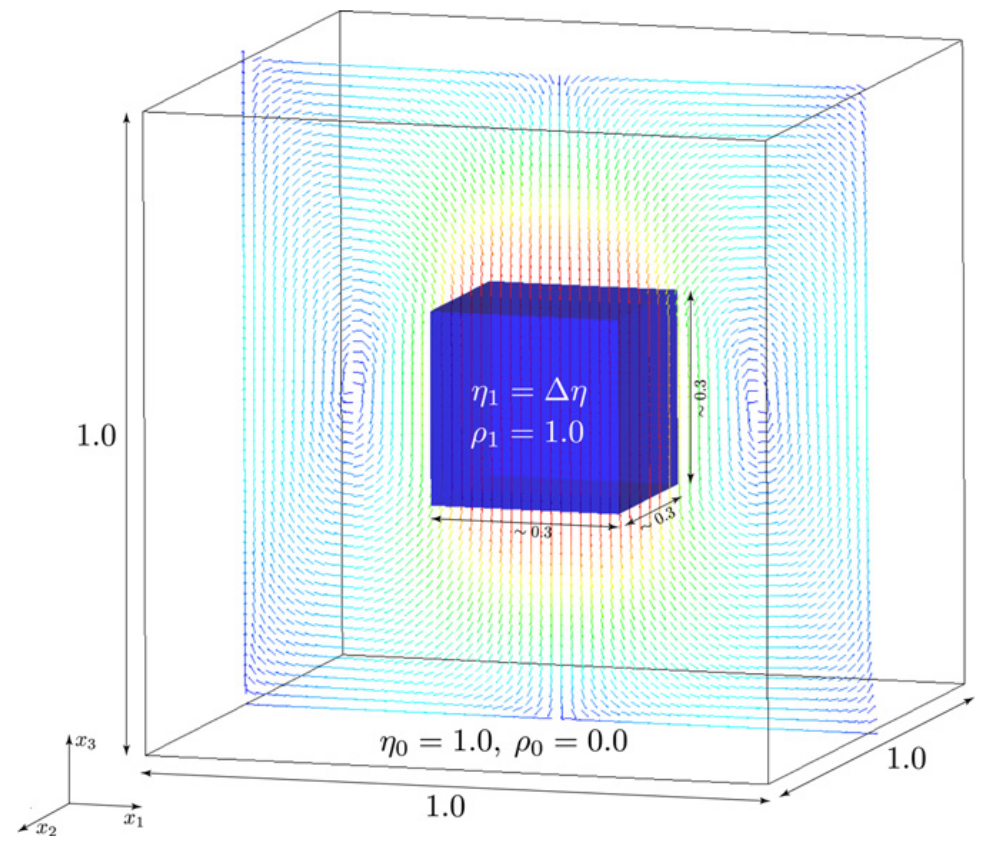
\includegraphics[width=8cm]{images/benchmark_sinker/fumt11}\\
{\scriptsize Simulation setup for the 3D falling block (SINKER) problem. The vectors represent computed flow.
Taken from \cite{fumt11}}
\end{center}



%......................................................
\subsubsection{The hot blob problem}\label{sec:hotblob}

This is a very similar setup as the 3D sinker from the same authors
with higher but more diffusive variation of viscosity.
The body force is given by $(0, 0, \beta T)$ and
where the temperature field $T$ is defined by $T = \exp  (-\gamma (x^2+y^2+(z-0.3)^2))$ 
with the constant parameters $\beta=10^6$ and $\gamma=200$. 
The temperature-dependent viscosity $\eta = \exp( -\alpha T)$ is employed with the parameter for viscosity
contrast $\alpha$.

\begin{center}
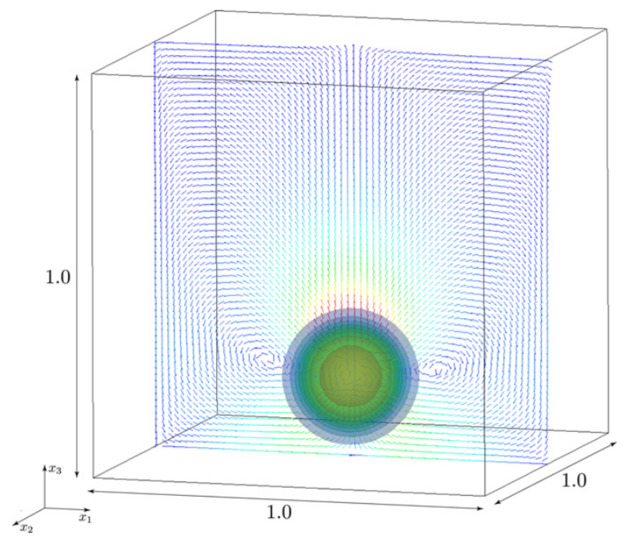
\includegraphics[width=8cm]{images/benchmark_hotblob/fumt11}\\
{\scriptsize Simulation setting of BLOB problem. Isosurface and vectors represent temperature field \\and computed flow respectively. Taken from \cite{fumt11}}
\end{center}



